% ---------------------------------------------------------------------------
%  Supplementary material. Every block here was lifted verbatim from the main
%  text when the manuscript was shortened; no number was changed. The
%  consistency test suite checks the main text and this file together, so a
%  figure that drifts fails whichever document it now lives in.
%  Compile: pdflatex supplementary.tex  (twice)
% ---------------------------------------------------------------------------
\documentclass[11pt,a4paper]{article}

\usepackage[margin=2.5cm]{geometry}
\usepackage{amsmath,amssymb}
\usepackage{newtxtext,newtxmath}
\usepackage{graphicx}
\usepackage{booktabs}
\usepackage[hidelinks]{hyperref}

\graphicspath{{../results/figures/}}

\renewcommand{\thesection}{S\arabic{section}}
\renewcommand{\thetable}{S\arabic{table}}
\renewcommand{\thefigure}{S\arabic{figure}}

\title{\bfseries Supplementary material\\
\large How much of the evidence for climate-driven dengue transmission
survives the analyst?\\A multiverse analysis of 221 outbreaks in 33 countries}

\author{Amna Dilber}
\date{}

\begin{document}
\maketitle

\noindent
Section numbers referenced from the main text. Every figure quoted here is
produced by a numbered pipeline step and stored in \texttt{results/tables/};
the test suite checks the main text and this document against those tables
together.

\section{How far the decomposition depends on the factor list}

More than the table above admits, and the honest version is worth more than the
comfortable one. The three designs are nested --- all contain the observation
model --- so agreement between them shows the answer survives adding cells to one
factor set, not that it survives choosing another. We therefore recomputed it
dropping each factor in turn, and over all 63 non-empty subsets of the six.

\begin{table}[htbp]
\centering
\caption{The within-outbreak share under alternative factor lists. The result is
load-bearing on the observation model and does not survive an adversarial choice
of factor list, which is stated here rather than left to be found.}
\begin{tabular}{lr}
\toprule
Factor list & Within-outbreak share \\
\midrule
All six factors & 76.5\% \\
\midrule
Dropping the fixed parameters & 76.7\% \\
Dropping the model structure & 73.6\% \\
Dropping the rainfall lag & 73.0\% \\
Dropping the temperature form & 71.4\% \\
Dropping the fraction of series fitted & 70.5\% \\
\textbf{Dropping the observation model} & \textbf{55.2\%} \\
\midrule
Median over all 63 subsets & 54.5\% \\
Best case for a sceptic (fixed parameters alone) & 2.3\% \\
\bottomrule
\end{tabular}
\end{table}

\begin{figure}[htbp]
\centering
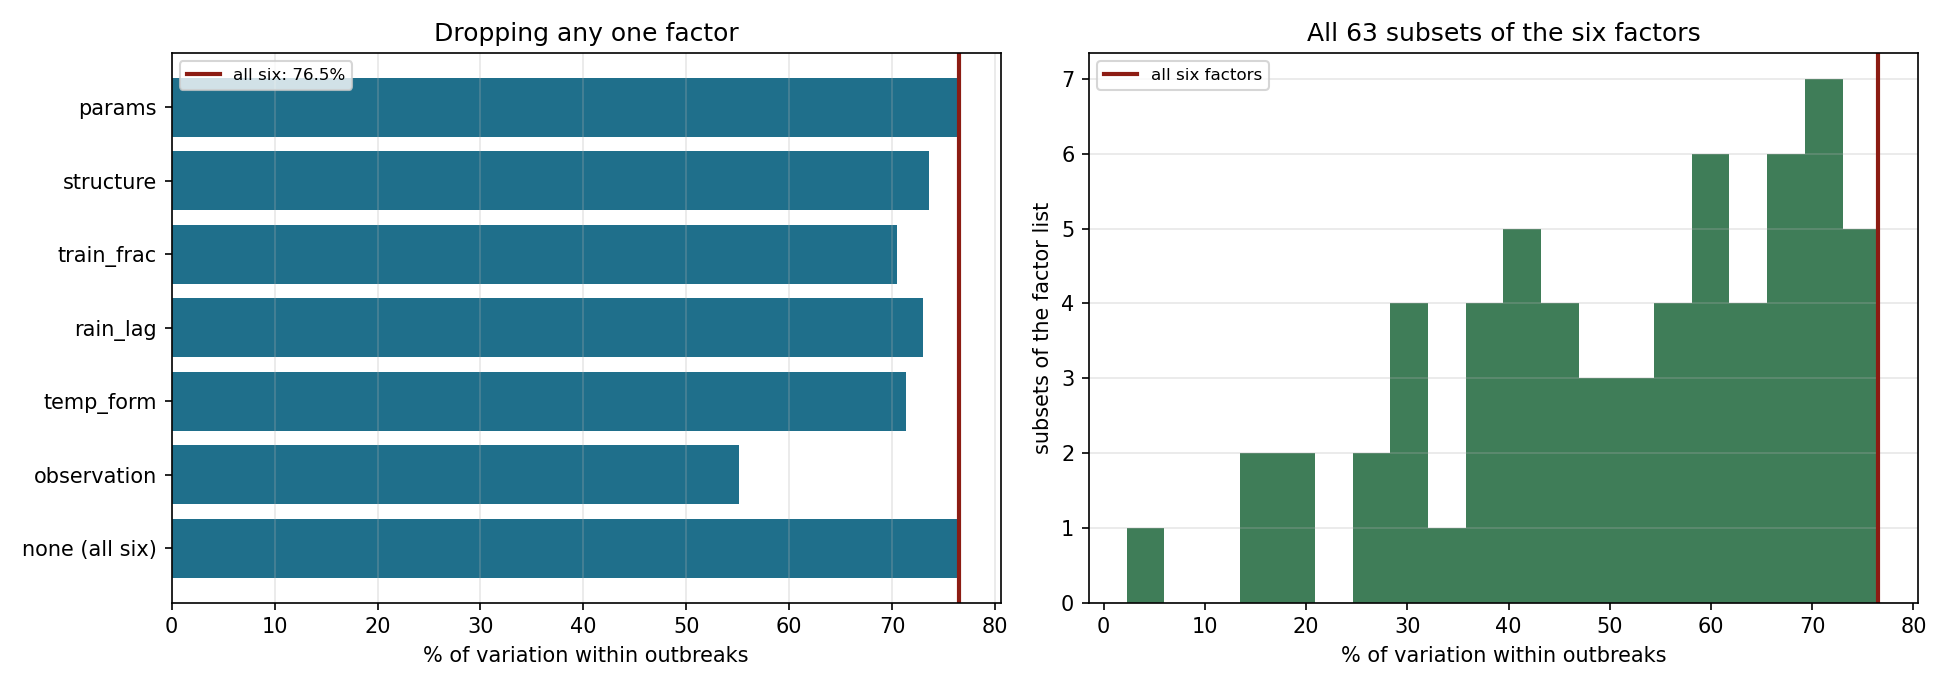
\includegraphics[width=\textwidth]{19_decomposition_robustness.png}
\caption{How far the headline depends on the factor list. Left: the
within-outbreak share when each factor is dropped in turn. Right: the same
quantity over all 63 non-empty subsets of the six factors. The claim is
load-bearing on the observation model and does not survive an adversarial choice
of factor list, which is why both panels are shown rather than the first alone.}
\label{fig:decomprobust}
\end{figure}

Removing any factor except the observation model costs at most six points.
Removing the observation model costs twenty-one, and the analytical share is then
55.2\% --- still a majority, but the claim is plainly load-bearing on that one
choice. A reader who regards the observation model as fixed by good practice
rather than chosen should read 55\%, and one who regards only the entomological
parameters as genuinely free should read 2.3\%.

We think the first two positions are the defensible ones, and the evidence for
that is in Section~3: the published review finds 18.3\% of models using Poisson
regression and 18.3\% linear regression, with the negative binomial not appearing
as a category. The observation model is not fixed by practice, because practice
has not fixed it.

One feature of the design was said to push the other way, and the claim was
never tested. Every combination within an outbreak is warm-started from a single
anchor fit and shares that fit's estimate of the dispersion, so the 144 analyses
are arguably more alike than 144 independent analysts would be, and earlier
drafts concluded that the share reported here is if anything an underestimate.
The optimiser check of Section~S5 refits seven outbreaks from ten
cold starts with no warm start, which measures the direction rather than arguing
it: pairwise disagreement is \textbf{33.4\%} as run and \textbf{32.9\%} cold.
Cold starts give slightly \emph{less} disagreement, not more. Seven outbreaks
settle nothing about the size, and the check varies the warm start but not the
shared dispersion, so one of the two mechanisms remains untested. We no longer
claim to know the sign.

This does not show that local context is irrelevant. It shows that context has
been asked to carry more than it can.

\section{The published moderator does not reproduce here}

The specific
contextual explanation on offer is that the association is strongest where
temperature varies most~\cite{kirk2024}. We tested its closest analogues on our
own data --- six descriptions of each outbreak's temperature regime against three
outcomes: the estimated Brière exponent, the share of analyses endorsing climate
forcing, and the disagreement between two of them. Eighteen correlations, so
about one would reach $p < 0.05$ by chance and reporting raw significance would
itself be the practice this paper measures.

Seven reach $p < 0.05$, against about one expected by chance, so the temperature
regime is not unrelated to what the analyses find. But every association is weak
--- no $|\rho|$ exceeds $0.22$ --- and \textbf{one survives control of the
false-discovery rate}: the estimated temperature exponent against the season's
temperature range, $\rho = -0.22$ ($q = 0.02$), whose sign is the wrong way round
for the hypothesis, the exponent being \emph{smaller} where temperature varies
more. The endorsement rate moves in the expected direction but does not survive
correction ($\rho = +0.15$, $q = 0.10$). Both facts belong in the same sentence:
there is something there, and it is small.

We do not read this as refuting the published result, which was computed on a
different quantity: they measured the strength of a statistical correlation
between incidence and temperature, we the exponent of a mechanistic response.
What it does establish is that the moderator is not recoverable from a design in
which the analysis is held fixed --- which is what it would have to be if it were
a property of dengue rather than of the estimates that reached print.

A mechanistic refinement we expected to do better also failed. Transmission
responds to temperature along a unimodal curve, so a season spent near the flat
optimum should offer nothing to detect while one crossing the steep flank offers
a great deal; the mean gradient traversed should therefore predict what the data
can support. It does not ($\rho = +0.13$, $q = 0.11$), and it is reported because
a study about undisclosed analytical choices does not get to drop the measure it
hoped would work.

\section{The instability is not specific to AIC}

AIC, BIC and the likelihood-ratio test are all thresholds on the same quantity,
placed at different points, so all three follow from what was already computed:
$\mathrm{AIC} = -2\log L + 2k$ recovers the log-likelihood, and $\Delta k = 2$ in
every comparison.

\begin{table}[htbp]
\centering
\caption{Instability under each criterion, used conventionally. All are thresholds
on $\Delta$AIC; the second column states where each one falls.}
\begin{tabular}{lrrr}
\toprule
Criterion & Equivalent to $\Delta$AIC $<$ & Unstable & 95\% CI \\
\midrule
AIC, sign & $0.00$ & 91.9\% & 88--96\% \\
Likelihood-ratio test, $p<0.05$ & $-1.99$ & 95.0\% & 91--98\% \\
BIC, sign (at the median 38 weeks) & $-3.28$ & 96.8\% & 95--99\% \\
Likelihood-ratio test, $p<0.01$ & $-5.21$ & 97.3\% & 95--99\% \\
\midrule
\textbf{AIC, abstain within $\pm 4$} & --- & \textbf{39.8\%} & 33--45\% \\
BIC, abstain within $\pm 4$ & --- & 90.5\% & 86--94\% \\
\bottomrule
\end{tabular}
\end{table}

Strictness makes matters worse, monotonically. The significance test an
epidemiologist would actually run is equivalent to a margin of about 2 and leaves
95\% of outbreaks unstable. A margin of 4 on the BIC scale, which sounds like the
same remedy, leaves 91\%, because BIC's additional penalty shifts the abstention
band off centre --- it abstains over $(-7.3, +0.7)$ rather than $(-4, +4)$, so one
side of the disagreement is still allowed to speak. The distinction that matters
is not how strict a rule is but whether it abstains symmetrically about zero.

\section{Why a small margin works and strictness does not}

Two facts hold simultaneously and sound contradictory until separated.

\textbf{The choices move the evidence enormously.} The range of $\Delta$AIC across
the 144 combinations of a single outbreak has a median of \textbf{804 AIC units}
(quartiles 140 to 11{,}105). The median $|\Delta\mathrm{AIC}|$ being interpreted as
evidence is 14.4. The analyst's own choices move the evidence by roughly
\textbf{fifty-six times} the size of the difference being read from it.

\textbf{Yet the dissent is marginal.} The margin needed to eliminate all
disagreement within a window has a median of 4.00, and in \textbf{60.2\%} of
outbreaks every dissenting combination does so on evidence weaker than
$\Delta$AIC $= 4$.

Here the six-factor design corrects a claim the smaller ones supported. On 48
combinations the margin needed was uncorrelated with how far the choices moved the
evidence, and dissent looked like a pure property of comparisons that were weak to
begin with. On 144 the correlation is $\rho = +0.61$ ($p = 4\times10^{-24}$): in
the remaining 39.8\% of outbreaks at least one dissenter is confident, and no band
around zero can reach it. What stays true is that such dissenters are few --- a
median of 3 of the 100 analyses still speaking.

Both hold because most of that enormous variation stays on one side of zero: it
changes how strong the evidence appears without changing which model it favours.
In three outbreaks in five, everything that does cross zero crosses it weakly, and
a band around zero reaches all of it. In the other two, something crosses
decisively and no band will ever reach it --- but when that happens the dissenter
is nearly alone, a median of 3 of the 100 analyses still speaking.

That is why a margin of 4 removes almost all pairwise disagreement (29.8\% to
4.0\%) while leaving 39.8\% of outbreaks with at least one dissenting cell. The
two figures describe the same fact from opposite ends and neither alone is honest:
the surviving disagreement is common across outbreaks and rare within them.

It also explains why a stricter threshold cannot help. A stricter rule is still a
rule with a boundary, and the confident dissent sits far from any boundary one
might choose; moving the boundary only changes which of the weak comparisons are
silenced.

We also tested and rejected a simpler explanation --- that instability tracks the
density of comparisons at the boundary. Scanning the threshold from $-14$ to $+2$
gives instability that runs backwards rather than forwards against the local
density ($\rho = -0.27$), so the hypothesis is not merely unsupported: it predicts
the wrong sign.

\begin{figure}[htbp]
\centering
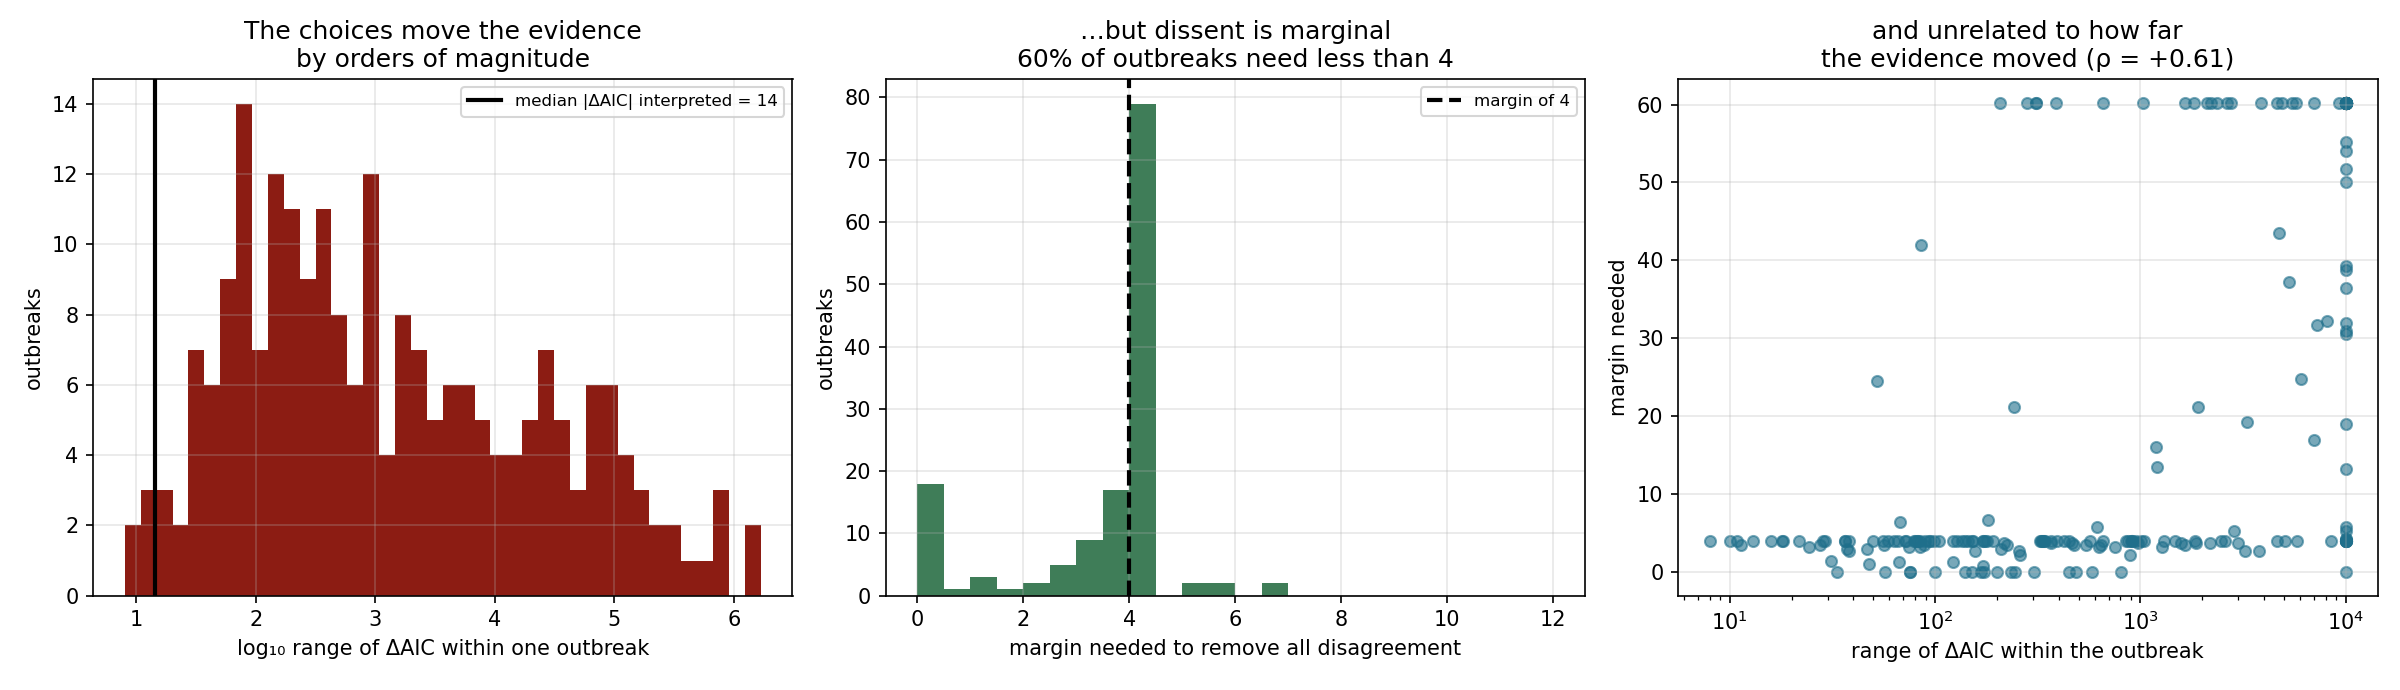
\includegraphics[width=\textwidth]{15_why_unstable.png}
\caption{Left: the range of $\Delta$AIC induced within a single outbreak by the
analysis choices, against the median difference interpreted as evidence. Centre:
the margin needed to remove all disagreement within a window. Right: the two are
unrelated.}
\end{figure}

\section{Further checks}

\textbf{Not a small-sample artefact.} By quartile of reported cases the unstable
share is 94.6\%, 90.9\%, 89.1\% and 92.7\%; by quartile of series length,
89.5\%, 93.2\%, 96.1\% and 88.9\%. Neither ordering is monotone and no quartile
falls below 88\%. This is not a problem of thin data.

\textbf{Not an artefact of our own selection rule.} This study applied a
peak-prominence threshold when choosing windows and must meet the standard it
sets for others. Recomputing the headline on progressively stricter subsets gives
91.9\%, 91.8\% and 94.1\% ($n=68$). Tightening our selection does not weaken the
result.

\textbf{The climate grid cell matters, and it is measured rather than conceded.}
A single representative point supplies the climate for a whole country or
province, which earlier versions of this study named as a limitation and did not
quantify. Forty outbreaks were therefore refitted under all 144 combinations at a
second point one degree of latitude away --- about 110 km, well inside the area
any of these case series aggregates over. Across 5{,}664 paired comparisons the
verdict changes in \textbf{12.0\%}, with the endorsement probability essentially
unmoved ($0.739 \to 0.737$). That places the climate location between the
covariate choices and the structural ones: above the transmission model, below
the observation model, and nowhere near the top.

Read it as an upper bound rather than an estimate. The offset is mechanical and
respects no terrain: in flat units the two series differ by a few tenths of a
degree, which is the intended comparison, but for Costa Rica they differ by
4.3\,\textdegree C because the shift crosses high ground --- a choice between two
climates rather than between two defensible stations for one population. The
alternative, hand-picking a second city per unit, would replace a reproducible
rule with a gazetteer of our own choices, which is not a substitution this study
is in a position to make quietly.

\textbf{Not optimiser noise.} The factorial used three multi-starts warm-started
from an anchor fit, a compromise made for runtime. If three starts sometimes miss
the optimum --- and miss it more often for the climate model, which has two extra
parameters --- then $\Delta$AIC would move for reasons unrelated to any analysis
choice. Seven outbreaks were therefore refitted twice under the 48-combination
design in place when the check was run: as run, and with ten cold restarts and no
warm start. The thorough setting does
find better optima, so the concern is not empty: it improves the climate fit in
6.1\% of comparisons and the constant fit in 3.3\%, and in one case by 1{,}656 AIC
units. But it changes the verdict in \textbf{0.6\%} of 329 paired comparisons,
against 8.3\% and 38.1\% for the weakest and strongest analysis factors
\emph{in that same 48-combination design} --- both bounds move when the factorial
grows, so the comparison has to be made within one design --- and
every one of the seven outbreaks is unstable under both settings. A more thorough
optimiser finds more, and what it finds does not move the conclusion. This check
is small --- seven outbreaks, run alongside the simulation study on the same
machine --- and is reported as a bound on optimiser noise rather than a precise
estimate of it.

\section{The Pakistani case study: what can be identified at all}

% ---------------------------------------------------------------------------
%  Moved out of the main text on review: it answers a different question from
%  the rest of the paper — not whether a conclusion is stable but whether the
%  underlying quantities are identifiable at all — and reads as a second study
%  when placed among the results.
% ---------------------------------------------------------------------------

% ===========================================================================
% ===========================================================================

The global study asks whether a conclusion is stable. It does not ask whether the
underlying quantities are identifiable, which we examined in detail on Pakistani
surveillance --- a national series covering the complete 2013 wave and provincial
series from 2021.

\textbf{Transmission is identified; catchment size often is not.} Profile
likelihoods~\cite{raue} bound $R_0$ and the population at risk in the longer windows, but in a
nineteen-week provincial window the population profile under the climate model is
flat across a twelvefold range, while the constant model determines it to within a
factor of two. Adding climate parameters to a short series destroys the
identifiability of a parameter the simpler model recovers.

\textbf{Spatial aggregation depresses $R_0$.} Fitting districts separately and
then fitting their sum gives different answers: a bias of $-2.2\%$ in one
province and $-28.8\%$ in another, where the aggregate estimate of 1.14 falls
below both constituent districts, 1.25 and 1.96. Component epidemics peak at
different times, and a homogeneously mixing model can only read the broader sum as
slower transmission.

\textbf{An independent check confirms it.} Bounding $R_0$ from the observed early
growth rate --- using no compartmental fit, and reporting both the fixed and
exponentially distributed generation-interval bounds --- gives 2.91--6.77
nationally against a fitted 1.37. Every fitted value falls below the corresponding
lower bound. A homogeneous model ties growth rate to final size through a single
$R_0$; these epidemics rise faster than their eventual size permits, which is the
same spatial heterogeneity seen from a second direction.

\textbf{And the explanation was tested, not asserted.} Spatial heterogeneity is
the natural account of both observations, but naming a mechanism is not
demonstrating it. A two-patch model was therefore fitted to the Khyber
Pakhtunkhwa \emph{aggregate} alone --- given no information about which districts
contributed, how many there were, or when each peaked. It beats the single-patch
fit by $\Delta\mathrm{AIC} = -8.6$, recovers transmission rates of 1.72 and 2.53
that bracket the two districts instead of falling below both, clears the
growth-rate lower bound the single-patch fit violated, and infers a 46-day offset
between its components. Three predictions of the heterogeneity account, each
checkable and each met, from a model that was told only the sum.

Fitted transmission rates from aggregated surveillance should therefore be read as
lower bounds, not as characteristic values.

\begin{thebibliography}{9}
\bibitem{kirk2024} D.~Kirk, S.~Straus, M.~L.~Childs et al., \emph{Temperature
impacts on dengue incidence are nonlinear and mediated by climatic and
socioeconomic factors: a meta-analysis}, PLOS Climate \textbf{3}(3), e0000152
(2024).
\bibitem{raue} A.~Raue, C.~Kreutz, T.~Maiwald, J.~Bachmann, M.~Schilling,
U.~Klingm\"uller and J.~Timmer, \emph{Structural and practical identifiability
analysis of partially observed dynamical models by exploiting the profile
likelihood}, Bioinformatics \textbf{25}(15), 1923--1929 (2009).
\end{thebibliography}

\end{document}
